\documentclass{article}

\usepackage{graphicx}
\usepackage{tikz}
\usepackage{tikzsymbols}
\usetikzlibrary{calc,patterns,shapes.geometric}
\pagestyle{empty}
\usepackage[margin=0pt]{geometry}
\geometry{papersize={14in,12in}}

\def\centerarc[#1](#2)(#3:#4:#5){\draw[#1] ($(#2)+({#5*cos(#3)},{#5*sin(#3)})$) arc (#3:#4:#5);}

\begin{document}
	\begin{figure}
		\centering
		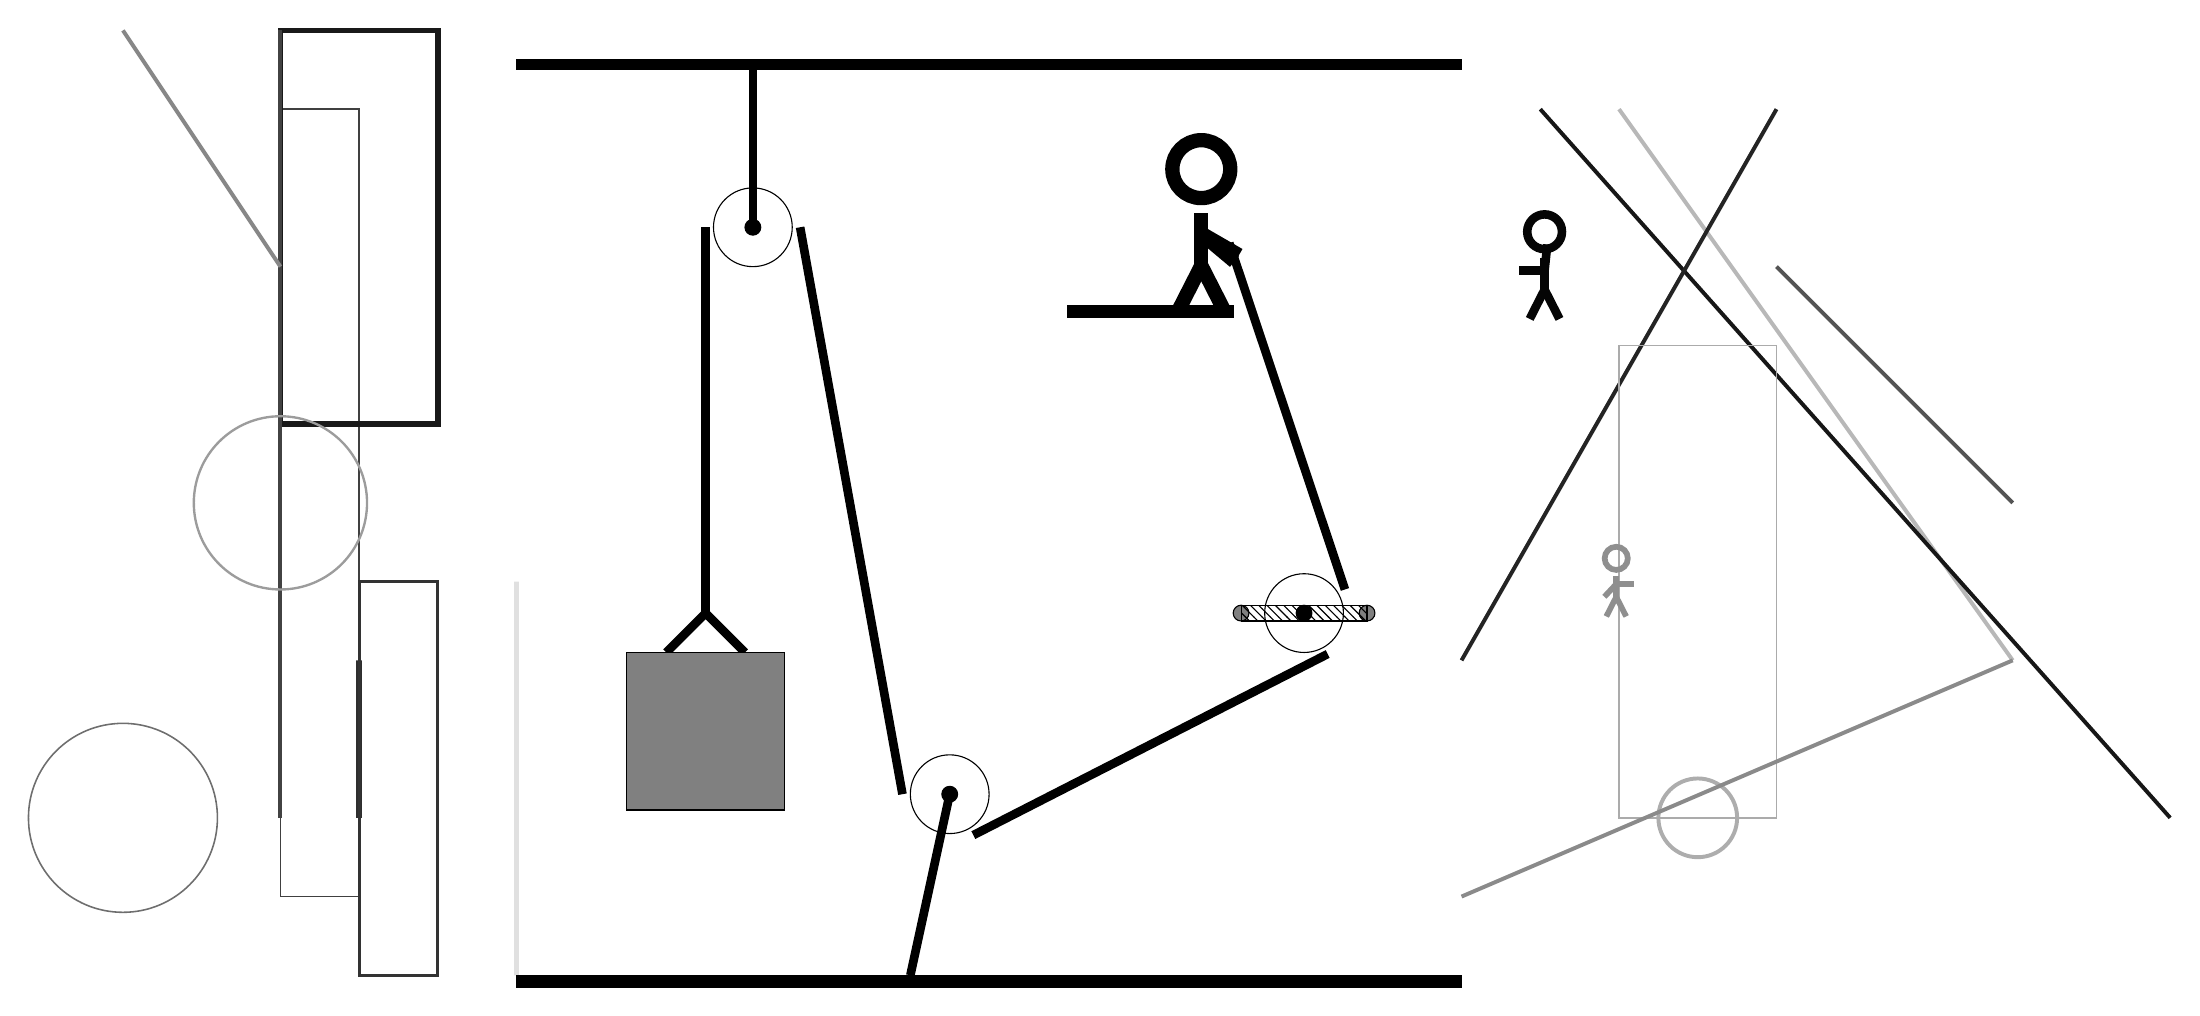
\begin{tikzpicture}
			%%%%% START %%%%%
			
			\draw[fill=black] (-2, 11.5) rectangle (10, 11.625);
			
			\draw (1, 9.5) circle (0.5);
			\draw[fill=black] (1, 9.5) circle (0.1);
			\draw[line width=1.1mm] (1, 11.5) -- (1, 9.5);
			
			\draw (3.5, 2.3) circle (0.5);
			\draw[fill=black] (3.5, 2.3) circle (0.1);
			\draw[line width=1.1mm] (3.5, 2.3) -- (3.0, 0);
			
			\draw [line width=0.2mm, color=black!57](-7, 2) circle (1.2);
			
			\draw[line width=0.5mm, color=black!28](12, 11) -- (17, 4);
			\draw[line width=0.5mm, color=black!91](11, 11) -- (19, 2);
			\draw[line width=0.7mm, color=black!82] (-4, 4) rectangle (-4, 2);
			\draw[line width=0.5mm, color=black!67](14, 9) -- (17, 6);
			\node[line width=0.7mm, color=black!98] at (11, 9) {\Strichmaxerl[6][0][84]};
			
			\draw [line width=0.5mm, color=black!32](13, 2) circle (0.5);
			\draw[line width=0.2mm, color=black!75] (-4, 1) rectangle (-5, 11);
			\draw[line width=0.6mm, color=black!12] (-2, 5) rectangle (-2, 0);
			
			\draw[line width=0.7mm, color=black!90] (-3, 7) rectangle (-5, 12);
			
			\draw[line width=0.5mm, color=black!74](-5, 12) -- (-5, 2);
			
			\draw[line width=0.5mm, color=black!86](10, 4) -- (14, 11);
			\draw[line width=0.2mm, color=black!33] (12, 8) rectangle (14, 2);
			
			\draw[line width=0.4mm, color=black!80] (-3, 0) rectangle (-4, 5);
			\draw[line width=0.5mm, color=black!46](10, 1) -- (17, 4);
			\node[line width=0.2mm, color=black!44] at (12, 5) {\Strichmaxerl[4][47][0]};
			
			\draw[line width=0.5mm, color=black!47](-7, 12) -- (-5, 9);
			\draw [line width=0.3mm, color=black!39](-5, 6) circle (1.1);
			
			\draw[fill=white](8, 4.6) circle (0.5);
			\draw[fill=black] (8, 4.6) circle (0.1);
			\draw[fill=black!50] (8.8, 4.6) circle (0.1);
			\draw[fill=black!50] (7.2, 4.6) circle (0.1);
			\draw[pattern=north west lines, pattern color=black] (7.2, 4.7) rectangle (8.8, 4.5);
			
			\draw[line width=1.1mm](-0.1, 4.1) --  (0.4, 4.6) -- (0.9, 4.1);
			\draw[fill=black!50] (-0.6, 4.1) rectangle (1.4, 2.1);
			
			\draw[line width=1.1mm](0.4, 9.5) -- (0.4, 4.6);
			\centerarc[line width=1.1mm](1, 9.5)(180:0:0.6)
			\draw[line width=1.1mm](1.6, 9.5) -- (2.9, 2.3);
			\centerarc[line width=1.1mm](3.5, 2.3)(180:300:0.6);
			\draw[line width=1.1mm](3.8, 1.7804) -- (8.3, 4.0804);
			\centerarc[line width=1.1mm](8, 4.6)(300:390:0.6);
			\draw[line width=1.1mm](8.5196, 4.9) -- (7.05, 9.3);
			
			\node at (6.75, 9.5) {\Strichmaxerl[10][-220][-30]};
			\draw[fill=black] (5, 8.5) rectangle (7.1, 8.35);
			
			\draw[fill=black] (-2, 0) rectangle (10, -0.15);
			
			%%%%% END %%%%%
		\end{tikzpicture}
	\end{figure}	
\end{document}